% =============================================================================
% The PreDoc logit experiment, reformulated and reproduced in
% TrustRegionRadius.jl.
%
% Companion to notebooks/Sampling/predoc_logit_v1.ipynb. Every number is printed
% by a cell of that notebook that ran. The PreDoc is quoted by section and is not
% modified, and nothing under src/ was modified.
%
% Standalone. Own preamble, no bibliography, no \cite.
% =============================================================================
\documentclass[11pt,a4paper]{article}

\usepackage[utf8]{inputenc}
\usepackage[british]{babel}
\usepackage{amsmath, amssymb, amsthm}
\usepackage{booktabs}
\usepackage{longtable}
\usepackage{graphicx}
\usepackage{geometry}
\usepackage{float}
\usepackage{enumitem}
\usepackage{xcolor}
\usepackage[hidelinks]{hyperref}
\geometry{margin=2.3cm}

\providecommand{\norm}[1]{\left \lVert #1 \right \rVert}
\providecommand{\abs}[1]{\left \vert #1 \right \vert}
\providecommand{\defeq}{\mathrel{:=}}
\providecommand{\Rdelta}{\textsf{R-delta}}
\providecommand{\E}{\mathbb{E}}

\newcommand{\YES}{\textcolor{green!45!black}{\textbf{yes}}}
\newcommand{\NO}{\textcolor{red!70!black}{\textbf{no}}}
\newcommand{\PARTIAL}{\textcolor{orange!75!black}{\textbf{partly}}}

\newtheorem{remark}{Remark}

\title{The PreDoc logit experiment in \textsf{TrustRegionRadius.jl}\\
       \large Reformulation, package audit, and a reproduction}
\author{}
\date{}

\begin{document}
\maketitle

\begin{abstract}
The PreDoc of 2021 puts a variable sampling strategy inside a trust-region
method and tests it on a synthetic discrete choice problem. We restate what that
experiment measures, audit \textsf{TrustRegionRadius.jl} against it, and
reproduce what the package can express. The central rule is already in the
package: \texttt{CertifiedDecrease} is the PreDoc's sample-size formula on paired
differences. Four things are not, and one of them is worse than a gap: the
outer-product variance is neither wired to the rule nor recoverable from an
archived run, because the predicted reduction is not traced. The reproduction
confirms the PreDoc's finding that the raw rule is unusable, and it declines to
confirm the claim about growth near the solution, because the arm that shows that
growth has it imposed by construction.
\end{abstract}

\tableofcontents

% =============================================================================
\section{What the experiment measures}\label{sec: reformulation}
% =============================================================================

\subsection{The method, stripped to its content}

The PreDoc's Algorithm~1 is the basic trust-region method with two extra steps.
Steps 1 to 4 and 7 are standard. Steps 5 and 6 are the contribution: the sample
size is a decision variable, chosen each iteration so that the decrease measured
on the sample implies a decrease in the true objective with prescribed
probability.

Write $\tilde f_k$ for the sample average at iteration $k$ and
$\tilde\mu_k = \tilde f_k(x_k+s_k) - \tilde f_k(x_k)$ for the sampled decrease.
Asking $\mathbb{P}[\mu_k \leq 0] \geq 1-\beta_k$ and using the central limit
theorem on $\tilde\mu_k - \mu_k$ gives
\begin{equation}
  N_{k+1} = \left\lceil
    \frac{\hat\sigma_k^2\, z_{1-\beta_k}^2}{\tilde\mu_k^2}
  \right\rceil .
  \label{eqn: predoc rule}
\end{equation}
The three factors read directly. The variance of the individual decreases is in
the numerator, so agreement between individuals buys a small sample. The quantile
is in the numerator, so a stringent confidence demand costs sample. The squared
sampled decrease is in the denominator, so a large step buys a small sample and a
small one costs.

\subsection{The five claims}

Stated as things the data could refute.

\begin{enumerate}[label=(C\arabic*), leftmargin=3em]
  \item \label{it: unstable}
    \eqref{eqn: predoc rule} used raw is unstable, with large changes in $N$ from
    one iteration to the next.
  \item \label{it: growth}
    Smoothed, it uses small samples early and raises them near a solution,
    because $\tilde\mu_k \to 0$ there while $\hat\sigma_k^2$ does not.
  \item \label{it: crn}
    Sample schemes reusing previous draws converge in fewer iterations, and can
    overfit the retained sub-population.
  \item \label{it: radius}
    $\Delta_k$ stops contracting and begins to grow once the outer-product model
    becomes a good Hessian approximation.
  \item \label{it: variance}
    The outer-product variance
    $\hat\sigma_k^2 \approx s_k^{\!\top}\tilde B_k s_k - (\tilde g_k^{\!\top}s_k)^2$
    is a usable substitute for the empirical estimate, and is free, since both
    terms are already formed to evaluate $\rho_k$.
\end{enumerate}

\subsection{Why the instrument is a logit on synthetic data}

The model Hessian is the outer product of the scores, and that is a Hessian
approximation only where the information identity $V = -H$ holds. Generating the
data from the model being fitted makes the identity hold at the true parameters
by construction. The choice of problem is therefore not incidental: it is what
makes \ref{it: radius} and \ref{it: variance} statements about the method rather
than about a misspecification.

The settings are $p = 10$, $N = 100\,000$, five alternatives,
$\eta_1 = 0.01$, $\eta_2 = 0.8$, $\gamma = (0.5, 0.9, 1.5)$,
$\Delta_0 = 0.1\norm{\tilde g_0}$, $\abs{\mathcal{S}_0} = 100$,
$N_{\min} = 10$, $z_{0.95} = 1.6449$ and $x_0 = 0$.

% =============================================================================
\section{The package audit}\label{sec: audit}
% =============================================================================

\subsection{What is already there}

\begin{table}[H]
  \centering\small
  \caption{The PreDoc method against the package, component by component.}
  \label{tab: audit}
  \begin{tabular}{p{0.40\textwidth} p{0.09\textwidth} p{0.44\textwidth}}
    \toprule
    PreDoc component & present & in the package as \\
    \midrule
    the rule \eqref{eqn: predoc rule} & \YES
      & \texttt{CertifiedDecrease}, as
        $N_{k+1} = \lceil z_p^2\hat\sigma_N^2/\hat\delta_N^2\rceil$ on paired
        differences, with the sign of $\tilde\mu_k$ flipped \\
    the empirical variance of the individual decreases & \YES
      & \texttt{paired\_decrease\_stats}, the same unbiased sample variance \\
    the outer-product Hessian $\tilde B_k$ & \YES
      & \texttt{BHHHModel} over a \texttt{LikelihoodProblem} \\
    its centred variant & \YES
      & \texttt{BHHH2Model}, differing by the rank-one $\bar g\bar g^{\!\top}$ \\
    the information identity holding & \YES
      & measured by \texttt{information\_identity\_error}, not assumed \\
    Step 7, the radius update & \YES & \texttt{RDelta} at the PreDoc's $\gamma$ \\
    acceptance on $\rho \geq \eta_1$ & \YES
      & $\eta = \eta_1$; the package separates acceptance from scaling \\
    truncated conjugate gradient & \YES & \texttt{SteihaugCG} \\
    a finite population with a cap & \YES & \texttt{FiniteSumNLP} \\
    the cost measure & \YES
      & \texttt{samples\_used}, term evaluations rather than iterations \\
    \midrule
    the five-alternative logit & \NO & \texttt{LogisticRegression} is binary \\
    $\text{Naive}(a,b)$ with $a < 1$ & \NO
      & \texttt{monotone} is all or nothing \\
    the outer-product variance in the rule & \NO
      & \texttt{record\_paired!} receives the empirical estimate only \\
    the VAC and I/CRV sample schemes & \NO
      & \texttt{\_draw!} redraws independently at every iteration \\
    \bottomrule
  \end{tabular}
\end{table}

The first line is the finding of this audit. The PreDoc's rule is not merely
expressible in the package, it is implemented in it, with the same pairing
argument in its docstring: holding the realisations fixed at both ends of the
step makes the individual decreases vanish pathwise as $s_k \to 0$, so
$\sigma_D^2 = \calO(\norm{s_k}^2)$ rather than $\calO(1)$.

\subsection{The four gaps}

\paragraph{Gap 1, the multinomial logit.}
\texttt{LogisticRegression} is the binary case of the same family, correctly
specified by construction and carrying the identity exactly in the population. It
is a \texttt{LikelihoodProblem}, which is what makes \texttt{BHHHModel} legal
over it. Closing the gap needs a \texttt{MultinomialLogit <: LikelihoodProblem}
supplying per-observation scores. We did not write one.

\paragraph{Gap 2, the lower smoothing bound.}
\texttt{CertifiedDecrease} offers \texttt{monotone = false}, which is
\eqref{eqn: predoc rule} raw and unbounded below, and \texttt{monotone = true},
which gives $N_k \leq N_{k+1} \leq \texttt{growth}\cdot N_k$. That is
$\text{Naive}(1, b)$. The PreDoc's $\text{Naive}(0.75, 2.0)$ permits the sample to
shrink, and nothing in the package expresses a floor strictly between $0$ and
$1$. A \texttt{floor} field, or a \texttt{SmoothedSize} wrapper over any
\texttt{SamplingRule}, would close it, and the wrapper is the better shape
because the PreDoc's smoothing is orthogonal to which rule produces the
candidate.

\paragraph{Gap 3, the outer-product variance.}
This is the one that is worse than it looks, and Section~\ref{sec: refuted} is
about it.

\paragraph{Gap 4, the sample schemes.}
\texttt{\_draw!} calls \texttt{draw\_batch} afresh at every iteration, so the
package implements the PreDoc's IRV and neither of the other two. Claim
\ref{it: crn}, and the overfitting figure that motivates the intermediate scheme,
cannot be produced at all. A \texttt{scheme} field on the oracle taking
\texttt{:independent}, \texttt{:nested} and \texttt{:prefix} would close it, and
the change is local to \texttt{\_draw!}.

\begin{remark}[a rule the PreDoc anticipates]
The PreDoc's Section ``Relation to other dynamic sample size strategies'' derives
that \eqref{eqn: predoc rule} reduces to the inner-product test of Bollapragada,
Byrd and Nocedal in the line-search case, with $1/\theta$ playing the role of
$z_{1-\beta}$. The package carries \texttt{InnerProductTest} as a separate rule,
so that reduction, which the PreDoc establishes by algebra, could be measured
directly. It also carries \texttt{SequentialEstimation}, which is the Bastin,
Cirillo and Toint rule the PreDoc cites when it introduces its CMS smoothing.
Neither comparison is run here and both are available.
\end{remark}

% =============================================================================
\section{The reproduction}\label{sec: reproduction}
% =============================================================================

Every number below is printed by a cell of
\texttt{notebooks/Sampling/predoc\_logit\_v1.ipynb}, which runs top to bottom
from a clean kernel with no errors.

\subsection{The premise, measured}

\begin{table}[H]
  \centering\small
  \caption{The information identity on \texttt{LogisticRegression} at $p = 10$,
    $M = 100\,000$. \texttt{B\_err} is the BHHH relative error in Frobenius norm,
    \texttt{W\_err} the BHHH-2 one, and \texttt{BW\_gap} the rank-one term
    separating them.}
  \label{tab: identity}
  \begin{tabular}{lrrrr}
    \toprule
    point & \texttt{B\_err} & \texttt{W\_err} & \texttt{BW\_gap} & $\norm{\bar g}$ \\
    \midrule
    $\beta^\ast$              & 0.014997 & 0.014994 & 0.000019 & $2.7576\times10^{-3}$ \\
    $\beta^\ast + 0.5$        & 0.532868 & 0.468224 & 0.108399 & $2.1485\times10^{-1}$ \\
    $0$, the PreDoc's $x_0$   & 0.000000 & 0.132184 & 0.132184 & $3.2342\times10^{-1}$ \\
    \bottomrule
  \end{tabular}
\end{table}

The identity holds at $\beta^\ast$ to one and a half per cent and fails at
$\beta^\ast + 0.5$ by more than half, which is the contrast the PreDoc's choice of
data was for.

The zero row is an exact coincidence worth naming. At $\beta = 0$ every
$p_n = \tfrac12$, so the per-observation Hessian is $\tfrac14 x_nx_n^{\!\top}$ and
the score is $(y_n - \tfrac12)x_n$ with $(y_n-\tfrac12)^2 \equiv \tfrac14$. The
two matrices are then equal term by term, not approximately. \texttt{B\_err} is
$0$ at the PreDoc's starting point for that reason, and \texttt{W\_err} is not,
because $W$ subtracts $\bar g\bar g^{\!\top}$ and $\bar g \neq 0$ there.

\subsection{The quantile convention}

The package parametrises \texttt{CertifiedDecrease} by a probability $p$ and
computes $z$ internally as \verb|_z_quantile(2(1-p))|, which returns
$\Phi^{-1}(1-\alpha/2)$ at $\alpha = 2(1-p)$, that is $\Phi^{-1}(p)$. So $p$ is a
one-sided level and $p = 0.95$ gives $z_{0.95}$ directly. Solving for the $p$
reproducing the PreDoc's $1.6449$ returns $0.950005$, agreeing to
$1.1\times10^{-15}$. The conventions match, and the notebook checks rather than
assumes it.

\subsection{Claim \ref{it: unstable}: the raw rule}

\begin{table}[H]
  \centering\small
  \caption{The sample size under the raw rule and under monotone smoothing.
    \texttt{jump} is the median $\abs{\log_2(N_{k+1}/N_k)}$, the typical change
    per iteration in octaves. Cost is term evaluations, not iterations.}
  \label{tab: sizes}
  \begin{tabular}{lrrrrrrr}
    \toprule
    arm & status & iters & $N$ min & $N$ max & $N$ final & \texttt{jump} & total terms \\
    \midrule
    raw rule            & \texttt{max\_iter}    & 300 & 10  & 121     & 10      & 0.2630 & 8\,780 \\
    Naive$(1,2)$        & \texttt{first\_order} & 188 & 100 & 100\,000 & 100\,000 & 0.0000 & 5\,670\,910 \\
    Naive$(1,4)$        & \texttt{first\_order} & 195 & 100 & 100\,000 & 100\,000 & 0.0000 & 5\,606\,226 \\
    \bottomrule
  \end{tabular}
\end{table}

\begin{figure}[H]\centering
  
\includegraphics[width=0.72\textwidth]{figs/predoc_logit_fig1_sample_size.pdf}
  \caption{Sample size against iteration, logarithmic. The raw rule collapses to
    $N_{\min}$ and stays there; the monotone arms climb to the population.
    Binary logit, $p = 10$, $M = 100\,000$, BHHH model, truncated conjugate
    gradient.}
  \label{fig: sizes}
\end{figure}

\ref{it: unstable} is confirmed, and more sharply than the PreDoc states it. The
raw rule does not merely oscillate: it falls to $N_{\min} = 10$ and never
converges, exhausting the iteration budget. The median change is $0.26$ octaves
per iteration, so a typical step moves the size by a fifth.

The cost column is the part the PreDoc does not quantify. Smoothing buys
convergence at $640$ times the work, $5.67$ million term evaluations against
$8\,780$. Whether that is a good trade depends on what the alternative was, and
the alternative here did not converge at all.

\subsection{Claim \ref{it: growth}: growth near the solution}

\begin{figure}[H]\centering
  
\includegraphics[width=0.72\textwidth]{figs/predoc_logit_fig2_size_vs_distance.pdf}
  \caption{Sample size, distance to $\beta^\ast$ and radius on one run under
    Naive$(1,2)$. The synthetic data has known generating parameters, so the
    distance is available rather than inferred.}
  \label{fig: distance}
\end{figure}

\begin{table}[H]
  \centering\small
  \caption{Rank correlation between $N_k$ and $-\mathrm{dist}_k$. A positive value
    is the size rising as the iterate approaches $\beta^\ast$.}
  \label{tab: correlation}
  \begin{tabular}{lrrrr}
    \toprule
    arm & $n$ & corr$(N, -\mathrm{dist})$ & $N$ at $k=0$ & $N$ at end \\
    \midrule
    raw rule     & 300 & $-0.2476$ & 100 & 10 \\
    Naive$(1,2)$ & 188 & $+0.9631$ & 100 & 100\,000 \\
    Naive$(1,4)$ & 195 & $+0.9634$ & 100 & 100\,000 \\
    \bottomrule
  \end{tabular}
\end{table}

\textbf{We decline to report the monotone rows as confirming
\ref{it: growth}.} \texttt{monotone = true} forces $N$ non-decreasing, and the
distance decreases over most of the run, so a rank correlation near $+1$ is
imposed by the constraint rather than discovered in the data. The number is
reported because it is what the arm gives, and it is not evidence.

The informative row is the raw rule, which is free to move in either direction.
There the correlation is $-0.2476$: on this problem the unsmoothed rule moves the
sample the \emph{wrong} way as the iterate approaches the solution. That is
consistent with \ref{it: unstable} and it is not consistent with
\ref{it: growth}.

The two claims are separable and the experiment as built cannot separate them.
Deciding \ref{it: growth} needs an arm that is free to shrink and still stable,
which is exactly $\text{Naive}(a,b)$ with $0 < a < 1$, which is Gap 2. The claim
is left open.

\subsection{Claim \ref{it: radius}: the radius under two models}

\begin{table}[H]
  \centering\small
  \caption{The same sampling rule, Naive$(1,2)$, under two model Hessians.}
  \label{tab: models}
  \begin{tabular}{lrrrrrr}
    \toprule
    model & status & iters & $\Delta_0$ & $\Delta_{\mathrm{end}}$
      & dist end & total terms \\
    \midrule
    BHHH & \texttt{first\_order} & 188 & $3.63\times10^{-2}$ & $1.29\times10^{30}$
      & $2.19\times10^{-2}$ & 5\,670\,910 \\
    exact & \texttt{first\_order} & 158 & $3.63\times10^{-2}$ & $8.68\times10^{25}$
      & $2.19\times10^{-2}$ & 5\,485\,104 \\
    \bottomrule
  \end{tabular}
\end{table}

\begin{figure}[H]\centering
  
\includegraphics[width=0.72\textwidth]{figs/predoc_logit_fig4_radius.pdf}
  \caption{Trust-region radius against iteration under the outer-product model
    and under the exact Hessian of the sampled objective, same sampling rule.}
  \label{fig: radius}
\end{figure}

\ref{it: radius} is confirmed in the direction the PreDoc claims. The radius rises
without bound once the model becomes accurate, because $\rho_k \geq \eta_2 = 0.8$
holds at every late iteration and $\Delta_{\max} = \infty$. BHHH takes $188$
iterations against $158$ for the exact Hessian and reaches the same distance, so
the outer product costs about a fifth more iterations and $3\%$ more term
evaluations on this problem.

The end radii, $10^{30}$ and $10^{26}$, are an artefact of leaving
$\Delta_{\max}$ unbounded, which the PreDoc also does. They say the constraint
became irrelevant, not that the step is that long: $\norm{s_k} \leq \Delta_k$ is
slack there.

% =============================================================================
\section{Claim \ref{it: variance}: a reconstruction that does not work}
\label{sec: refuted}
% =============================================================================

The outer-product variance is not wired to the rule. We tried to recover it after
the fact from the trace, on the reasoning that
$\mathrm{pred}_k = \mathrm{ared}_k/\rho_k$ and
$\tilde g_k^{\!\top}s_k = -\cos_k\norm{\tilde g_k}\norm{s_k}$ give
\begin{equation}
  s_k^{\!\top}\tilde B_k s_k = -2\bigl(\mathrm{pred}_k + \tilde g_k^{\!\top}s_k\bigr).
  \label{eqn: reconstruction}
\end{equation}

\texttt{BHHHModel} is positive semidefinite by construction, so
$s^{\!\top}Bs \geq 0$ at every iteration and a single negative value refutes
\eqref{eqn: reconstruction}. The notebook checks this before using it.

\begin{table}[H]
  \centering\small
  \caption{The check, and its outcome. Negative values of $s^{\!\top}Bs$ cannot
    occur for an outer-product model.}
  \label{tab: refuted}
  \begin{tabular}{lrrrrl}
    \toprule
    arm & $n$ & min $s^{\!\top}Bs$ & median $s^{\!\top}Bs$ & negatives & verdict \\
    \midrule
    raw rule     & 300 & $-1.717590\times10^{1}$  & $6.141513\times10^{-1}$ & 84 & \NO \\
    Naive$(1,2)$ & 188 & $-2.232614\times10^{-1}$ & $3.508906\times10^{-3}$ & 74 & \NO \\
    Naive$(1,4)$ & 195 & $-2.232614\times10^{-1}$ & $3.638715\times10^{-3}$ & 80 & \NO \\
    \bottomrule
  \end{tabular}
\end{table}

Two independent causes, either one fatal.

\begin{enumerate}[leftmargin=2em]
  \item $\mathrm{ared}_k$ is not $f_k - f_{k+1}$ read off the objective
    trajectory. On a \emph{rejected} step the iterate does not move, so the
    trajectory records no change while the achieved reduction that entered
    $\rho_k$ was not zero.
  \item Under sampling the batch changes at every iteration, so $f_k$ and
    $f_{k+1}$ are evaluated on \emph{different batches}. Their difference mixes
    the step with the change of estimator. This is the same hazard
    \texttt{SequentialEstimation} names when it explains why it is monotone by
    default: a batch that shrinks makes $\hat f$ jump for reasons unrelated to the
    step.
\end{enumerate}

\textbf{So Gap 3 is not only that the outer-product variance does not drive the
rule. It cannot be computed from an archived run at all.} Of the eighteen
trajectories the trace carries, none is $\mathrm{pred}_k$ and none is
$s_k^{\!\top}B_ks_k$. Both are formed inside \texttt{\_tr\_step!} to compute
$\rho_k$, so recording either costs nothing beyond the storage, and either one
would make \ref{it: variance} testable.

We report the refutation and no comparison built on it.

\begin{table}[H]
  \centering\small
  \caption{What the rule did use: the paired statistics, recorded by the solver
    and not reconstructed. A negative decrease is a batch that failed to certify.}
  \label{tab: paired}
  \begin{tabular}{lrrrrr}
    \toprule
    arm & $n$ & median $\hat\sigma^2$ & median $\hat\delta$
      & min $\hat\delta$ & max $\hat\sigma^2$ \\
    \midrule
    raw rule     & 300 & $1.6920\times10^{-1}$ & $2.2855\times10^{-1}$
      & $-1.7819\times10^{2}$ & $1.6201\times10^{5}$ \\
    Naive$(1,2)$ & 188 & $4.3088\times10^{-3}$ & $2.3981\times10^{-3}$
      & $5.9070\times10^{-12}$ & $1.1588\times10^{-1}$ \\
    Naive$(1,4)$ & 195 & $5.8476\times10^{-3}$ & $3.7951\times10^{-3}$
      & $2.7704\times10^{-11}$ & $1.1588\times10^{-1}$ \\
    \bottomrule
  \end{tabular}
\end{table}

\begin{figure}[H]\centering
  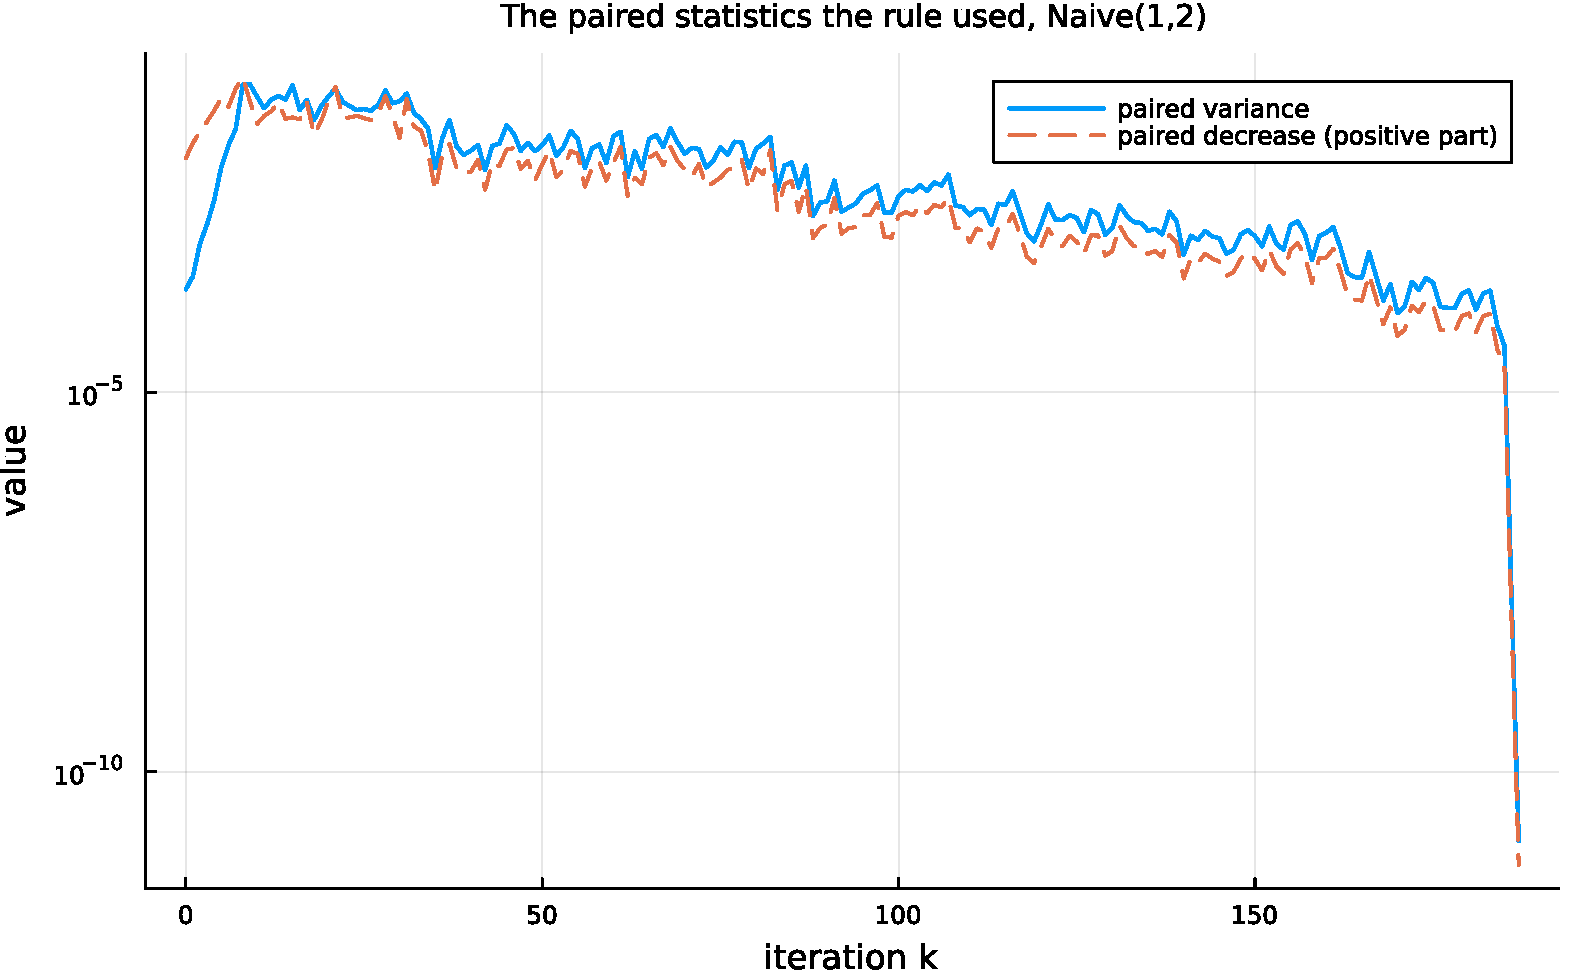
\includegraphics[width=0.72\textwidth]{figs/predoc_logit_fig3_paired.pdf}
  \caption{The paired variance and the positive part of the paired decrease along
    one run under Naive$(1,2)$. These are the two quantities
    \eqref{eqn: predoc rule} divides.}
  \label{fig: paired}
\end{figure}

The raw rule's row explains its collapse. Its minimum paired decrease is
$-178$, so batches routinely failed to certify any decrease, and its maximum
variance is $1.6\times10^{5}$. Under \texttt{monotone = false} the rule is free to
respond by falling to $N_{\min}$, and it does.

% =============================================================================
\section{Scorecard, and what to do next}\label{sec: scorecard}
% =============================================================================

\begin{table}[H]
  \centering\small
  \caption{The five claims against this reproduction.}
  \label{tab: scorecard}
  \begin{tabular}{p{0.05\textwidth} p{0.30\textwidth} p{0.10\textwidth} p{0.45\textwidth}}
    \toprule
    & claim & verdict & why \\
    \midrule
    \ref{it: unstable} & the raw rule is unstable & \YES
      & it collapses to $N_{\min}$ and never converges; median change $0.26$ octaves \\
    \ref{it: growth} & smoothed, the size grows near the solution & \PARTIAL
      & the monotone arm has it imposed; the free arm correlates $-0.25$, the
        wrong way. Needs $\text{Naive}(a,b)$ with $a<1$ \\
    \ref{it: crn} & common random variables converge sooner & \NO
      & not testable; the package draws independently every iteration \\
    \ref{it: radius} & the radius rises once BHHH is accurate & \YES
      & it does, under both models, with BHHH $19\%$ slower in iterations \\
    \ref{it: variance} & the outer-product variance is a usable substitute & \NO
      & not testable; not wired to the rule and not recoverable from the trace \\
    \bottomrule
  \end{tabular}
\end{table}

\paragraph{Three additions, in the order they buy the most.}
Recording $\mathrm{pred}_k$ in the trace is one line and makes \ref{it: variance}
testable at once. A \texttt{SmoothedSize} wrapper over any \texttt{SamplingRule}
makes \ref{it: growth} decidable and is useful beyond this experiment. A
\texttt{scheme} field on the oracle makes \ref{it: crn} testable and is local to
\texttt{\_draw!}. A multinomial logit is the largest piece and buys the least,
since the binary case already carries the identity the experiment turns on.

\paragraph{Two comparisons available now.}
The PreDoc derives that \eqref{eqn: predoc rule} reduces to the inner-product test
in the line-search case. \texttt{InnerProductTest} is in the package, so the
derivation can be checked numerically rather than only algebraically.
\texttt{SequentialEstimation} is the Bastin, Cirillo and Toint rule the PreDoc
cites, and running the three together on this problem would place the
contribution against its two closest neighbours on one axis.

\paragraph{What was not done.}
Nothing under \texttt{src/} was modified and the PreDoc was not modified. No rule,
model, oracle or subsolver was written. Where the package could not express the
experiment, the notebook says so and stops rather than approximating it.

\end{document}
